\documentclass{article}
% For math environments
\usepackage{amsmath, amsfonts}
% For links
\usepackage[hidelinks]{hyperref}
% So space it put between paragraphs
\usepackage{parskip}
% For figures
\usepackage{tikz}
% Set the margins to not be ridiculous
\usepackage[margin=0.75in]{geometry}
% For multiple columns
\usepackage{multicol}
% For controlling enum/itemize spacing and indentation
\usepackage{enumitem}

% For tikz plots
\usepackage{pgfplots}
% This isn't needed but avoids a compiler warning
\pgfplotsset{compat=1.16}

% Allow multi-line equations to be broken across pages
\allowdisplaybreaks

% Use @ as a letter
\makeatletter

% Scale down all tikz coordinates while maintaining font size
\tikzset{every picture/.style={scale=0.45, every picture/.style={}}}


% Macros
% Monospace code
\def\code#1{\texttt{#1}}

% Greek letters
\def\a{\alpha}
\def\b{\beta}
\def\g{\gamma}
\def\d{\delta}
\def\D{\Delta}

% Some common sets
\def\es{\varnothing}
\def\ints{{\mathbb{Z}}}

% Commands that make life easier
\newcommand\gath[1]{\begin{gather} #1 \end{gather}}
\newcommand\gaths[1]{\begin{gather*} #1 \end{gather*}}
\newcommand\ali[1]{\begin{align} #1 \end{align}}
\newcommand\parens[1]{\left( #1 \right)}
\newcommand\squares[1]{\left[ #1 \right]}
\newcommand\braces[1]{\left\{ #1 \right\}}
\newcommand\angles[1]{\left\langle #1 \right\rangle}
\newcommand\deriv[2]{\frac{d #1}{d #2}}
\newcommand\abs[1]{\left| #1 \right|}
\newcommand\floor[1]{\left\lfloor #1 \right\rfloor}
\newcommand\ceil[1]{\left\lceil #1 \right\rceil}
\DeclareMathOperator{\lcm}{lcm}
\def\non{\nonumber \\}
\newcommand\unit[1]{~\mathrm{#1}}
\newcommand\combos[2]{{}_{#1}C_{#2}}

% Set stuff
\def\ss{\subseteq}

% Multiline equation space
\def\mlesp{\hspace{1.2cm}}

% For grid diagrams
\newcommand\gridbox[3]{\draw (#1,#2) rectangle (#1+1,#2+1) node[pos=.5] {#3};}
\newcommand\gridboxh[3]{\draw[fill=red!20] (#1,#2) rectangle (#1+1,#2+1) node[pos=.5] {#3};}
\newcommand\gridboxb[3]{\draw[fill=black] (#1,#2) rectangle (#1+1,#2+1) node[pos=.5] {#3};}
\newcommand\gridsym[3]{\node at (#1+0.5,#2+0.5) {$#3$};}
\newcommand\gridblank[2]{\filldraw[draw=gray, color=gray] (#1,#2) rectangle (#1+1,#2+1);}
\newcommand\gridcirc[2]{\draw (#1 + 0.5,#2 + 0.5) circle (0.25);}
\newcommand\cwlab[3]{
  \def\dd{0.15}
  \draw (#1 + \dd - 0.03, #2 + 1 - \dd) node {\scriptsize #3};
}

\def\bbw{3.5}
\def\bbh{2}
\newcommand\bigbox[3]{\draw (#1*\bbw,#2*\bbh) rectangle (#1*\bbw+\bbw,#2*\bbh+\bbh) node[pos=.5] {#3};}
\newcommand\bbtextr[3]{\node[right] at (#1*\bbw,#2*\bbh+0.5*\bbh) {#3};}
\newcommand\bbtextb[3]{\node[align=center] at (#1*\bbw+0.5*\bbw,#2*\bbh+0.5*\bbh) {#3};}

% Box puzzle stock answer
\newcommand\boxans[1]{
  Logic was used to deduce the solution:

  #1

  This was verified using Python as well as shown to be unique with a brute force approach.
}

% Standard crossnumber grid
\newcommand\crossnumstd[9]{
  \begin{center}
    \begin{tikzpicture}[scale=2]
      \gridbox{0}{2}{#1}
      \gridbox{1}{2}{#2}
      \gridbox{2}{2}{#3}
      \gridbox{0}{1}{#4}
      \gridbox{1}{1}{#5}
      \gridbox{2}{1}{#6}
      \gridbox{0}{0}{#7}
      \gridbox{1}{0}{#8}
      \gridbox{2}{0}{#9}

      % Labels
      \cwlab{0}{2}{1}
      \cwlab{1}{2}{2}
      \cwlab{2}{2}{3}
      \cwlab{0}{1}{4}
      \cwlab{0}{0}{5}
    \end{tikzpicture}
  \end{center}
}

% Multiple numbers
\newcommand\mn[1]{$#1$'s}

% Commands for problems
\newcommand\problem[4]{
\section*{#1}

\textbf{Question:} #3

\textbf{Answer:} #2

\textbf{Explanation:} #4
}
\newcommand\aproblem[4]{\problem{Dec #1}{#2}{#3}{#4}}
\newcommand\cproblem[4]{\problem{Problem #1}{#2}{#3}{#4}}

\newcommand\xref@advent[2]{#1 Advent, Dec~#2 problem}
\newcommand\xref@card[2]{#1 Christmas Card, Problem #2}

% For answered verified with Python
\newcommand{\verified}{This was verified with a brute-force Python program.}

\def\advent@xxi@i{
  The geometric mean of a set of $n$ numbers can be computed by multiplying together all the numbers then computing the $n$th root of the result.

  The factors of $4$ are $1$, $2$ and $4$. The geometric mean of these is 2.

  The factors of $6$ are $1$, $2$, $3$, and $6$. The geometric mean of these is $\sqrt{6}$.

  The geometric mean of all the factors of today's number is $22$.
}

\def\advent@xxi@ii{
  The number $7n$ has $37$ factors (including $1$ and the number itself).
  How many factors does $8n$ have?
}

\def\advent@xxi@iii{
  If you write out the numbers from $1$ to $1000$ (inclusive), how many times will you write the digit $0$?
}

\def\advent@xxi@iv{
  Put the digits $1$ to $9$ (using each digit exactly once) in the boxes so that the sums are correct.
  The sums should be read left to right and top to bottom ignoring the usual order of operations.
  For example, $4 + 3 \times 2$ is $14$, not $10$.
  Today's number is the product of the numbers in the red boxes.

  \grid@advent@xxi@iv{}{}{}{}{}{}{}{}{}
}

\def\advent@xxi@v{
  How many different isosceles triangles are there whose perimeter is $50$ units, and whose area is an integer number of units squared?

  (Two triangles that are rotations, reflections and translations of each other are counted as the same triangle. Triangles with an area of 0 should not be counted.)
}

\def\advent@xxi@vi{
  When $12345$ is divided by today's number, the remainder is $205$.
  When $6789$ is divided by today's number, the remainder is $112$.
}

\newcommand\dec@ai{0.30901699437494745}
\newcommand\dec@aii{0.8090169943749475}
\newcommand\dec@bi{0.5877852522924731}
\newcommand\dec@bii{0.9510565162951535}
\newcommand\decagon[5]{
  \def\ai{\dec@ai*#3+#1}
  \def\aii{\dec@aii*#3+#1}
  \def\bi{\dec@bi*#3+#2}
  \def\bii{\dec@bii*#3+#2}
  \draw (#3+#1, #2) -- (\aii, \bi) -- (\ai, \bii) -- (-\ai, \bii) -- (-\aii, \bi) -- (-#3+#1, #2) -- (-\aii, -\bi) -- (-\ai, -\bii) -- (\ai, -\bii) -- (\aii, -\bi) -- cycle;
  \fill[fill=red] (-\ai, -\bii) -- (#4*#3+#1, #5*#3+#2) -- (\ai, -\bii) -- cycle;
}
\def\advent@xxi@vii{
  The picture below shows eight regular decagons.
  In each decagon, a red triangle has been drawn with vertices at three of the vertices of the decagon.

  \begin{center}
    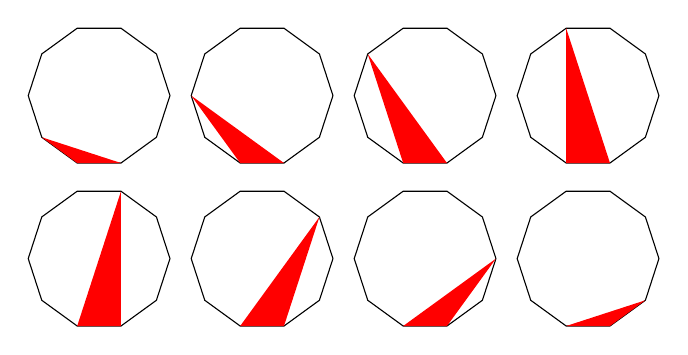
\begin{tikzpicture}
      \def\dr{2}
      \def\spc{2.3*\dr}

      \decagon{0*\spc}{\spc}{\dr}{-\dec@aii}{-\dec@bi}
      \decagon{1*\spc}{\spc}{\dr}{-1}{0}
      \decagon{2*\spc}{\spc}{\dr}{-\dec@aii}{\dec@bi}
      \decagon{3*\spc}{\spc}{\dr}{-\dec@ai}{\dec@bii}

      \decagon{0*\spc}{0}{\dr}{\dec@ai}{\dec@bii}
      \decagon{1*\spc}{0}{\dr}{\dec@aii}{\dec@bi}
      \decagon{2*\spc}{0}{\dr}{1}{0}
      \decagon{3*\spc}{0}{\dr}{\dec@aii}{-\dec@bi}
    \end{tikzpicture}
  \end{center}

  The area of each decagon is $240$.
  What is the total area of all the red triangles?
}

\def\advent@xxi@viii{
  The sum of three integers is $51$.
  The product of the same three integers is $836$. What is the product of largest integer and the second-largest integer?
}

\def\advent@xxi@ix{
  Eve writes down a sequence of consecutive positive integers (she writes more than one number).
  The sum of the numbers Eve has written down is $844$.
  Today's number is the smallest integer that Eve has written down.
}

\def\advent@xxi@x{
  Put the digits $1$ to $9$ (using each digit exactly once) in the boxes so that the sums are correct.
  Today's number is the largest number you can make using the digits in the red boxes.

  \grid@advent@xxi@x{}{}{}{}{}{}{}{}{}
}

\def\advent@xxi@xi{
  The integers are written in a triangle as shown below:
  \begin{center}
    \begin{tabular}{ccccccc}
         &    &    & 1    &    &    &    \\
         &    & 2  & 3    & 4  &    &    \\
         & 5  & 6  & 7    & 8  & 9  &    \\
      10 & 11 & 12 & 13   & 14 & 15 & 16 \\
         &    &    & etc. &    &    &
    \end{tabular}
  \end{center}
  Today's number appears directly above the number $750$ in the triangle of integers.
}

\def\advent@xxi@abgrid{
  \begin{center}
    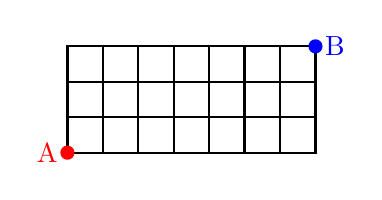
\begin{tikzpicture}
      \def\gs{1}
      % Grid
      \foreach \i in {0,...,6}{
          \foreach \j in {0,...,2}{
              \draw[thick] (\i * \gs, \j * \gs) rectangle (\i * \gs + \gs, \j * \gs + \gs);
            }
        }
      % Points
      \fill[color=red] (0, 0) circle (0.2) node[color=red,left] {A};
      \fill[color=blue] (7*\gs, 3*\gs) circle (0.2) node[color=blue,right] {B};
    \end{tikzpicture}
  \end{center}
}
\def\advent@xxi@xii{
  You start at the point marked A in the picture below. You want to get to the point marked B.
  You may travel \textbf{to the right} or \textbf{upwards} along the black lines.

  \advent@xxi@abgrid

  Today's number is the total number of possible routes to get from A to B.
}

\def\advent@xxi@xiii{
  The diagram below shows three circles and two triangles.
  The three circles all meet at one point.
  The vertices of the smaller red triangle are at the centers of the circles.
  The lines connecting the vertices of the larger blue triangle to the point where all three circles meet are diameters of the three circles.

  \begin{center}
    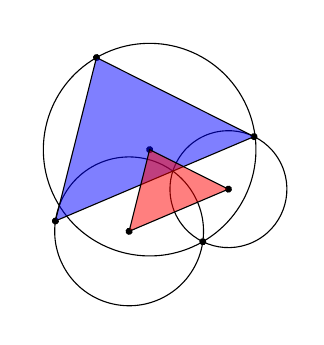
\begin{tikzpicture}[rotate=30,transform shape]
      \def\bcr{3}
      \def\scr{0.55*\bcr}
      \def\sca{34}
      \def\mcr{0.7*\bcr}
      \def\mca{142}
      \def\pr{0.1}

      % Circles
      \draw (0, \bcr) circle (\bcr);
      \draw (\sca: \scr) circle (\scr);
      \draw (\mca: \mcr) circle (\mcr);

      % Points
      \fill (0, 0) circle (\pr);
      \fill (0, \bcr) circle (\pr);
      \fill (0, 2*\bcr) circle (\pr);
      \fill (\sca: \scr) circle (\pr);
      \fill (\sca: 2*\scr) circle (\pr);
      \fill (\mca: \mcr) circle (\pr);
      \fill (\mca: 2*\mcr) circle (\pr);

      % Triangles
      \draw[fill=blue,fill opacity=0.5] (\mca: 2*\mcr) -- (0, 2*\bcr) -- (\sca: 2*\scr) -- cycle;
      \draw[fill=red,fill opacity=0.5] (\mca: \mcr) -- (0, \bcr) -- (\sca: \scr) -- cycle;
    \end{tikzpicture}
  \end{center}

  The area of the smaller red triangle is $226$.
  What is the area of the larger blue triangle?
}

\def\advent@xxi@xiv{
  You start at the point marked A in the picture below.
  You want to get to the point marked B.
  You may travel \textbf{to the right}, \textbf{upwards}, or \textbf{to the left} along the black lines, but you cannot pass along the same line segment more than once.

  \advent@xxi@abgrid

  Today's number is the total number of possible routes to get from A to B.
}

\newcommand\pyramid@advent@xxi@xvi[6]{
  \begin{center}
    \begin{tabular}{cccccc}
      (row 1) &    &    & #1   &    &    \\
      (row 2) &    & #2 &      & #3 &    \\
      (row 3) & #4 &    & #5   &    & #6 \\
              &    &    & etc. &    &
    \end{tabular}
  \end{center}
}
\def\advent@xxi@xv{
  The odd numbers are written in a pyramid.

  \pyramid@advent@xxi@xvi{1}{3}{5}{7}{9}{11}

  What is the mean of the numbers in the 19th row?
}

\newcommand\grid@advent@xxi@xvi[9]{
  \begin{center}
    \begin{tikzpicture}[scale=2]
      \gridbox{0}{2}{#1}
      \gridbox{1}{2}{#2}
      \gridbox{2}{2}{#3}
      \gridbox{0}{1}{#4}
      \gridbox{1}{1}{#5}
      \gridbox{2}{1}{#6}
      \gridbox{0}{0}{#7}
      \gridbox{1}{0}{#8}
      \gridbox{2}{0}{#9}

      % Labels
      \cwlab{0}{2}{1}
      \cwlab{1}{2}{2}
      \cwlab{2}{2}{3}
      \cwlab{0}{1}{4}
      \cwlab{0}{0}{5}
    \end{tikzpicture}
  \end{center}
}
\def\advent@xxi@xvi{
  Each clue in this crossnumber is formed of two parts connected by a logical connective: AND means that both parts are true; NAND means that at most one part is true; OR means that at least one part is true; NOR means that neither part is true; XOR means that exactly one part is true; XNOR means that either both parts are false or both parts are true.
  No number starts with $0$.

  \begin{multicols}{2}
    \grid@advent@xxi@xvi{}{}{}{}{}{}{}{}{}

    \columnbreak

    \begin{enumerate}
      \item \textbf{1A} is a palindrome XNOR \textbf{1D} is a palindrome.
      \item \textbf{1A} is greater than $350$ NOR \textbf{1D} is less than $150$.
      \item \textbf{3D} is odd NAND \textbf{4A} and \textbf{2D} are equal.
      \item \textbf{3D} is prime XOR \textbf{5A} is odd.
      \item \textbf{4A} is a cube AND \textbf{2D} is a cube.
      \item The sum of the digits of \textbf{3D} is $2$ OR the sum of the digits of \textbf{5A} is $5$.
      \item Today's number is \textbf{1D}.
    \end{enumerate}
  \end{multicols}
}

\def\advent@xxi@xvii{
  The digital product of a number is computed by multiplying together all of its digits. For example, the digital product of $6273$ is $252$.

  Today's number is the smallest number whose digital product is $252$.
}

\def\advent@xxi@xviii{
  Put the digits $1$ to $9$ (using each digit exactly once) in the boxes so that the sums are correct.
  The sums should be read left to right and top to bottom ignoring the usual order of operations.
  For example, $4 + 3 \times 2$ is $14$, not $10$.
  Today's number is the product of the numbers in the red boxes.

  \grid@advent@xxi@xviii{}{}{}{}{}{}{}{}{}
}

\def\advent@xxi@xix{
  The equation $352x^3 - 528x^2 + 90 = 0$ has three distinct real-valued solutions.

  Today's number is the number of integers $a$ such that the equation $352x^3 - 528x^2 + a = 0$ has three distinct real-valued solutions.
}

\def\advent@xxi@xx{
  What is the area of the largest area triangle that has one side of length $32$ and one side of length $19$?
}

\newcommand\grid@advent@xxi@xxi[9]{
  \begin{center}
    \begin{tikzpicture}
      \bigbox{0}{3}{#1}
      \bigbox{1}{3}{#2}
      \bigbox{2}{3}{#3}
      \bbtextr{3}{3}{\textbf{today's number}}

      \bigbox{0}{2}{#4}
      \bigbox{1}{2}{#5}
      \bigbox{2}{2}{#6}
      \bbtextr{3}{2}{prime}

      \bigbox{0}{1}{#7}
      \bigbox{1}{1}{#8}
      \bigbox{2}{1}{#9}
      \bbtextr{3}{1}{square}

      \bbtextb{0}{0}{cube}
      \bbtextb{1}{0}{odd}
      \bbtextb{2}{0}{multiple\\of $11$}
    \end{tikzpicture}
  \end{center}
}
\def\advent@xxi@xxi{
  Arrange the digits $1$–$9$ (using each digit exactly once) so that the three digit number in: the middle row is a prime number; the bottom row is a square number; the left column is a cube number; the middle column is an odd number; the right column is a multiple of $11$.
  The $3$-digit number in the first row is today's number.

  \grid@advent@xxi@xxi{}{}{}{}{}{}{}{}{}
}

\def\advent@xxi@xxii{
  There are $12$ ways of placing $2$ tokens on a $2 \times 4$ grid so that no two tokens are next to each other horizontally, vertically or diagonally:

  \begin{center}
    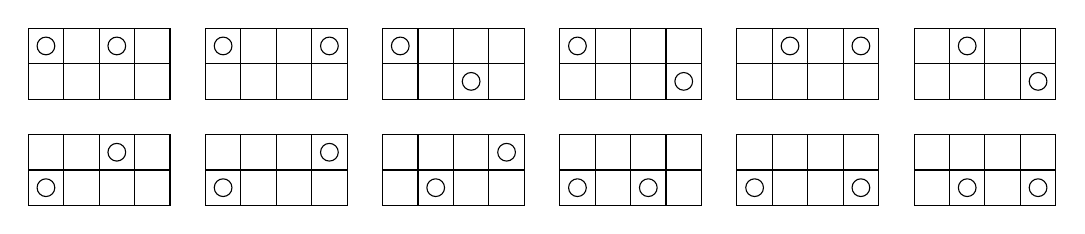
\begin{tikzpicture}
      % Draw all the grids
      \foreach \gi in {0,1}{
          \foreach \gj in {0,...,5}{
              \foreach \i in {0,1}{
                  \foreach \j in {0,...,3}{
                      \gridbox{5*\gj + \j}{3*\gi + \i}{}
                    }
                }
            }
        }

      % Place token circles
      \gridcirc{0}{4}
      \gridcirc{2}{4}
      \gridcirc{5}{4}
      \gridcirc{8}{4}
      \gridcirc{10}{4}
      \gridcirc{12}{3}
      \gridcirc{15}{4}
      \gridcirc{18}{3}
      \gridcirc{21}{4}
      \gridcirc{23}{4}
      \gridcirc{26}{4}
      \gridcirc{28}{3}
      \gridcirc{0}{0}
      \gridcirc{2}{1}
      \gridcirc{5}{0}
      \gridcirc{8}{1}
      \gridcirc{11}{0}
      \gridcirc{13}{1}
      \gridcirc{15}{0}
      \gridcirc{17}{0}
      \gridcirc{20}{0}
      \gridcirc{23}{0}
      \gridcirc{26}{0}
      \gridcirc{28}{0}
    \end{tikzpicture}
  \end{center}

  Today's number is the number of ways of placing $2$ tokens on a $2 \times 21$ grid so that no two tokens are next to each other horizontally, vertically or diagonally.
}

\def\advent@xxi@xxiii{
  I draw the parabola $y = x^2$ and mark points on the parabola at $x = 17$ and $x = -6$.
  I then draw a straight line connecting these two points.

  At which value of $y$ does this line intercept the $y$-axis?
}

\def\advent@xxi@xxiv{
  The digital product of a number is computed by multiplying together all of its digits.
  For example, the digital product of $1522$ is $20$.

  How many $12$-digit numbers are there whose digital product is $20$?
}

\def\card@xxi@i{
  What is the sum of all the odd integers between $0$ and $30$?
}

\def\card@xxi@ii{
  What is the sum of all the odd integers between $0$ and $5668$?
}

\def\card@xxi@iii{
  What is the smallest integer with a digital sum of $28$ and a digital product of $10000$?
}

\def\card@xxi@iv{
  What is the smallest integer with a digital sum of $41$ and a digital product of $432000$?
}

\def\card@xxi@v{
  What is the area of the largest area dodecagon that will fit inside a circle with area $111185 \pi$?
}

\def\card@xxi@vi{
  What is the area of the largest area heptagon that will fit inside a semicircle with area $115185 \pi$?
}

\def\card@xxi@vii{
  How many terms are there in the (simplified) expansion of $(x + y + z)^2$?
}

\def\card@xxi@viii{
  How many terms are there in the (simplified) expansion of $(x + y + z)^{41172}$?
}

\def\card@xxi@ix{
  What is the largest integer that cannot be written as $4a + 5b$ for non-negative integers $a$ and $b$?
}

\def\card@xxi@x{
  What is the largest integer that cannot be written as $83409a + 66608b$ for non-negative integers $a$ and $b$?
}

\def\card@xxi@xi{
  How many positive integers are there below $100$ whose digits are all non-zero and different?
}

\def\card@xxi@xii{
  How many positive integers are there whose digits are all non-zero and different?
}

\def\card@xxi@xiii{
  What is the only integer for which taking the geometric mean of all its factors (including $1$ and the number itself) gives $2$?
}

\def\card@xxi@xiv{
  What is the only integer for which taking the geometric mean of all its factors (including $1$ and the number itself) gives $25$?
}

\input{boxes}

\begin{document}

\title{MS Scroggs Advent Calendar 2020 Answers}
\author{Dan Whitman}
\date{}

\maketitle

Answers: \href{https://www.mscroggs.co.uk/puzzles/advent2020}{https://www.mscroggs.co.uk/puzzles/advent2020}

\aproblem{1}{195}{\advent@xx@i}{
The number of $r$-digit numbers formed using these digits is the number of permutations of the 5 digits, selecting $r$ of them.
Hence the total number of numbers is the sum of these permutations from 1-digit numbers to 5-digit numbers:
\gath{
\sum_{r=1}^5 {}_5 P_r = \sum_{r=1}^5 \frac{5!}{(5-r)!} = 325 \,.
}
If interested only in the odd numbers, the least significant digit must be chosen from the 3 odd digits (1, 3, and 5) whereas the rest are chosen normally from the remaining digits.
Thus the total number of odd numbers is reasoned to be
\gath{
  \sum_{r=1}^5 \frac{3 \cdot 4!}{5 - r} = 195 \,.
}

This answer was also verified using a brute force Python program.
}

\aproblem{2}{124}{\advent@xx@ii}{
  For a square with sides of length $s$, the smallest circle in which the square can fit is reasoned to have a radius of $r = s / \sqrt{2}$.
  For a circle of radius $r$, the smallest square into which the circle can fit is reasoned to have sides of $s = 2r$.

  So, in our case, we have an initial square of area $a = 62$ and sides of $s = \sqrt{a}$.
  Hence the smallest circle containing this square has a radius of
  \gath{
    r = \frac{s}{\sqrt{2}} = \frac{\sqrt{a}}{\sqrt{2}} = \sqrt{\frac{a}{2}} \,.
  }
  The smallest square containing this circle then has sides of
  \gath{
    S = 2r = 2 \sqrt{\frac{a}{2}} = \sqrt{2a} \,.
  }
  Hence the area of this square is
  \gath{
    A = S^2 = 2a = 124 \,.
  }
}

\aproblem{3}{321}{\advent@xx@iii}{
  \boxans{\gridsol@advent@xx@iii}
}

\aproblem{4}{371}{\advent@xx@iv}{
  Solved this using a brute force Python program.
}

\aproblem{5}{103}{\advent@xx@v}{
  For $n$ dice, the minimum possible sum is $n$ when they all roll a one.
  The maximum number is $6n$ when they all roll a six.
  Every sum $s$ such that $n \leq s \leq 6n$ is possible and occurs some number of times in the $6^n$ possible dice combinations.
  Obviously the sums $s = n$ and $s = 6n$ each occur only once.
  Let $N_n(s)$ be the number of combinations that sum $s$ occurs in the rolls of $n$ dice, which is of course directly related to the probability of that sum occurring.
  Though I was unable to prove it, some numerical experiments showed that all the values of $s$ are symmetric such that
  \gath{
    N_n(n + i) = N_n(6n - i)
  }
  for all integer $0 \leq i \leq 5n$.

  Letting $a = 200$ and $b = 521$, there must then be some integers $n$ and $i$ such that
  \ali{
    n + i &= a \non
    6n -i &= b
  }
  since these sums have the same probability.
  Thus this linear system can be solved:
  \gath{
    \begin{bmatrix}
      1 & 1  \\
      6 & -1
    \end{bmatrix}
    \begin{bmatrix}
      n \\ i
    \end{bmatrix}
    =
    \begin{bmatrix}
      a \\ b
    \end{bmatrix} \,.
  }
  Doing so results in $n = 103$ and $i = 97$, where of course $n$ is the number of dice and so is our answer.
}

\aproblem{6}{192}{\advent@xx@vi}{
  First, we notice that, if $N$ is the number of indistinguishable tokens used, then both the example and our actual problem are $2 \times 2N$ grids.
  We can use this to our advantage by considering only this special case.
  So first let $f(N)$ denote the number of valid placements of $N$ tokens on a $1 \times 2N$ grid.
  For a single token we have only a $1 \times 2$ grid, in which there are clearly only $f(1) = 2$ possible placements.
  Next consider a $1 \times 2N$ grid, where we divide the grid in to $N$ distinct $1 \times 2$ regions horizontally.
  Because we have $N$ tokens, it follows that the $n$th token is confined to the $n$th $1 \times 2$ region in order for all of the tokens to fit validly on the board.

  If the first token is positioned on the left side of its $1 \times 2$ grid as illustrated below,

  \newcommand\gridboxo[4]{\draw[fill=gray!20] (#1,#2) rectangle (#1+#3,#2+1) node[pos=.5] {#4};}
  \begin{center}
    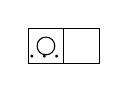
\begin{tikzpicture}
      \gridbox{0}{0}{}
      \gridcirc{0}{0}
      \gridbox{1}{0}{}
      \gridboxo{2}{0}{1}{}
      \gridboxo{3}{0}{2}{$\cdots$}
      \gridboxo{5}{0}{1}{}
    \end{tikzpicture}
  \end{center}

  then the remaining $N-1$ tokens can be placed freely on the remaining $1 \times 2(N-1)$ grid so that there are $f(N-1)$ of these placements.
  However, if the first token is on the right of its $1 \times 2$ grid, then this forces all of the remaining tokens to the right side of their $1 \times 2$ grids in order for the board to be valid

  \begin{center}
    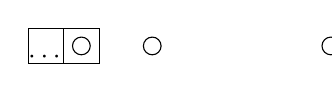
\begin{tikzpicture}
      \gridbox{0}{0}{}
      \gridbox{1}{0}{}
      \gridcirc{1}{0}
      \gridboxo{2}{0}{1}{}
      \gridboxo{3}{0}{1}{}
      \gridcirc{3}{0}
      \gridboxo{4}{0}{2}{$\cdots$}
      \gridboxo{6}{0}{1}{}
      \gridboxo{7}{0}{1}{}
      \gridcirc{7}{0}
    \end{tikzpicture}
  \end{center}

  and so clearly there is only one valid placement for this case.
  Thus the number of configurations for $N$ tokens is simply $f(N) = f(N-1) + 1$.
  So $f$ is defined by the following recursive relationship:
  \ali{
    f(1) &= 2 \non
    f(N) &= f(N-1) + 1 \,.
  }
  We can easily prove that $f(N) = N + 1$ by induction.
  First, clearly $f(1) = 1 + 1 = 2$ as required.
  Now suppose that $f(N) = N + 1$ so that
  \gath{
    f(N+1) = f((N+1) - 1) + 1 = f(N) + 1 = (N + 1) + 1 \,,
  }
  which shows the induction step.

  Now, one property that a general $2 \times m$ grid has is that, whether a token is on the upper or lower row, it blocks exactly the same spaces.
  Because of this, for a given valid placement on a $1 \times 2N$ grid with $N$ tokens, there are exactly $2^N$ valid placements on a $2 \times 2N$ grid, one for every combination where the tokens can either be on the upper or lower row.
  Think of binary numbers where a token on the lower row is a 0 and a token on the upper row is a 1.
  Thus the total number of valid placements for a $2 \times 2N$ grid with $N$ tokens is
  \gath{
    g(N) = 2^N f(N) = 2^N (N + 1) \,.
  }
  So, for the given example, we have $g(2) = 12$ as expected, and for the actual problem our answer is $g(5) = 192$.

  This answer was also verified using a brute force Python program.
}

\aproblem{7}{315}{\advent@xx@vii}{
First, in general for non-negative integers $b \geq a$, we have
\gath{
  \sum_{i=a}^b i = \sum_{i=0}^b i - \sum_{i=0}^{a-1} i = \frac{b(b+1)}{2} - \frac{a(a-1)}{2} = \frac{1}{2} [b(b+1) - a(a-1)] \,,
}
noting that this is valid even when $a = 0$ since this causes the second term to vanish.
We also have
\gath{
  \sum_{i=a}^b i^2 = \sum_{i=0}^b i^2 - \sum_{i=0}^{a-1} i^2 = \frac{b(b+1)(2b+1)}{6} - \frac{a(a-1)(2a-1)}{6} = \frac{1}{6} [b(b+1)(2b+1) - a(a-1)(2a - 1)] \,,
}
which is also valid when $a = 0$ for the same reason.

Now consider the general case of all the dominoes with integers running from $a$ to $b$ (inclusive) so that of course $b \geq a$.
Then the number of such dominoes is reasoned to be
\ali{
  N(a, b) &= \sum_{i=a}^b \sum_{j=i}^b 1 = \sum_{i=a}^b (b - i + 1) = (b + 1)\sum_{i=a}^b 1 - \sum_{i=a}^b i \non
  &= (b + 1) (b - a + 1) - \frac{1}{2} [b(b+1) - a(a-1)] \non
  &= \frac{1}{2}[(b+1)(2b - 2a + 2 - b) + a(a+1)] \non
  &= \frac{1}{2}[(b+1)(b - 2a + 2) + a(a+1)] \,,
}
where the indices $i$ and $j$ are the numbers appearing on the domino for each term.
Since this is the case, the sum of the numbers on all $N(a,b)$ of the dominoes is reasoned to be
\ali{
S(a, b) &= \sum_{i=a}^b \sum_{j=i}^b (i+j) = \sum_{i=a}^b \parens{i \sum_{j=i}^b 1 + \sum_{j=i}^b j} \non
&= \sum_{i=a}^b \parens{i (b - i + 1) + \frac{1}{2}[b(b+1) - i(i-1)]} \non
&= \frac{1}{2} \sum_{i=a}^b [2bi - 2i^2 + 2i + b(b+1) - i^2 + i] \non
&= \frac{1}{2} \sum_{i=a}^b [(2b + 3)i - 3i^2 + b(b+1)] \non
&= \frac{1}{2} \left[(2b + 3) \sum_{i=a}^b i - 3 \sum_{i=a}^b i^2 + b(b+1) \sum_{i=a}^b 1\right] \non
&= \frac{1}{2} \{(2b+3)\frac{1}{2}[b(b+1) - a(a-1)] - \frac{1}{2}[b(b+1)(2b+1) - a(a-1)(2a-1)] \non
&\mlesp + b(b+1)(b-a+1)\} \non
&= \frac{1}{4} \{b(b+1)[(2b+3) - (2b+1) + 2(b - a + 1)] + a(a-1)[(2a-1) - (2b + 3)]\} \non
&= \frac{1}{4} [2b(b+1)(b - a + 2) + 2a(a-1)(a - b - 2)] \non
&= \frac{1}{2} [b(b+1)(b - a + 2) + a(a-1)(a - b - 2)] \non
&= \frac{1}{2}(b - a + 2)[b(b+1) - a(a-1)] \,.
}
As expected, for the example, we get $N(0, 4) = 15$ dominoes with a sum of $S(0,4) = 60$ using these formulas.
For the actual problem we get $N(5,10) = 21$ dominoes and a sum of $S(5, 10) = 315$, the latter of which is of course our answer.
}

\aproblem{8}{121}{\advent@xx@viii}{
  In octal, 11 is $n = 9$ decimal so that $n^2 = 81$ (decimal).
  This is $n^2 = 121$ in octal, which is our answer.

  This was verified with Python, which easily does octal conversions.
}

\aproblem{9}{144}{\advent@xx@ix}{
  \boxans{\gridsol@advent@xx@ix}
}

\aproblem{10}{888}{\advent@xx@x}{
  The smallest such number is $888 = 37 \times 24$.
  This was solved with Python.
}

\aproblem{11}{216}{\advent@xx@xi}{
  \def\ra{r_A}
  \def\rb{r_B}
  \def\ba{b_A}
  \def\bb{b_B}

  Suppose we have the following variables:
  \begin{center}
    \begin{tabular}{cl}
      $\ra$ & Number of red cards initially in pile A   \\
      $\ba$ & Number of black cards initially in pile A \\
      $\rb$ & Number of red cards initially in pile B   \\
      $\bb$ & Number of black cards initially in pile B
    \end{tabular}
  \end{center}
  and let $m = 108$ be the number of red cards that were transferred.

  First, the number of total red and black cards must be equal, i.e.
  \gath{
    \ra + \rb = \ba + \bb \,, \label{eqn:pxi:rbs}
  }
  and of course the total number of cards is
  \gath{
    n = \ra + \rb + \ba + \bb = 2(\ra + \rb) = 2(\ba + \bb) \,. \label{eqn:pxi:n}
  }
  Since initially two thirds of the cards in pile A are red, this results in
  \gath{
    \frac{\ra}{\ra + \ba} = \frac{2}{3} \non
    3\ra = 2\ra + 2\ba \non
    \ra = 2 \ba \,. \label{eqn:pxi:ra}
  }
  Similarly, after the move, two thirds of the cards in pile $B$ are red so that
  \gath{
    \frac{\rb + m}{\rb + \bb + m} = \frac{2}{3} \non
    3\rb + 3m = 2\rb + 2\bb + 2m \non
    \rb = 2\bb - m \,. \label{eqn:pxi:rb}
  }
  Substituting \eqref{eqn:pxi:ra} and \eqref{eqn:pxi:rb} into \eqref{eqn:pxi:rbs} results in
  \gath{
    \ba + \bb = \ra + \rb = 2\ba + 2\bb - m \non
    \ba + \bb = m \,.
  }
  Hence the total number of cards is $n = 2(\ba + \bb) = 2m = 216$ by \eqref{eqn:pxi:n}, which is of course our answer.

  Note that this also means that the total number of red cards is $\ra + \rb = \ba + \bb = m$.
  Since $m$ cards were transferred from pile A to pile B, it then has to be that $\ra = m$ and $\rb = 0$ so that evidently pile B contained only black cards before the move, and pile A contained only black cards after the move.
  From \eqref{eqn:pxi:ra} and \eqref{eqn:pxi:rb} it follows that $\ba = \bb = m/2 = 54$ so that pile A before the move is identical to pile $B$ after the move and vice versa.

  This answer was verified with Python.
}

\aproblem{12}{334}{\advent@xx@xii}{
  First, divide the region \emph{outside} the blue quadrilateral into the following labeled squares and right triangles:

  \begin{center}
    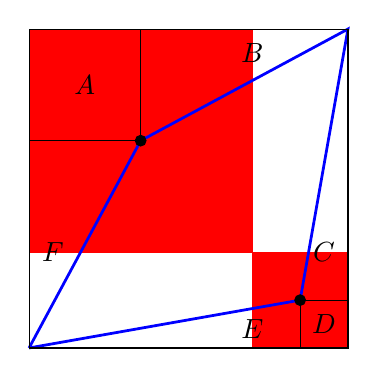
\begin{tikzpicture}
      \def\bss{9}
      \def\mpt{0.7}
      \coordinate (A) at (\mpt * \bss / 2, -\mpt * \bss / 2);
      \coordinate (B) at (\mpt * \bss /2 + \bss/2, -\mpt * \bss /2 - \bss/2);
      \filldraw[draw=black, color=red] (0, 0) rectangle (\mpt * \bss, -\mpt * \bss);
      \filldraw[draw=black, color=red] (\mpt * \bss, -\mpt * \bss) rectangle (\bss, -\bss);
      \draw[line width=1, color=blue] (0,-\bss) -- (A) -- (\bss, 0) -- (B) -- (0, -\bss);
      \draw[fill=black] (A) circle (0.15);
      \draw[fill=black] (B) circle (0.15);
      \draw (0,0) rectangle (\bss,-\bss);

      % Draw regions
      \draw (0,0) rectangle (A);
      \draw (B) rectangle (\bss, -\bss);

      % Region labels
      \draw (\mpt * \bss/4, -\mpt * \bss/4) node {$A$};
      \draw (\mpt * \bss, -0.075 * \bss) node {$B$};
      \draw (\bss - 0.075*\bss, -\mpt * \bss) node {$C$};
      \draw (0.75*\bss + \mpt * \bss / 4, -0.75*\bss - \mpt * \bss / 4) node {$D$};
      \draw (\mpt * \bss, -\bss + 0.06*\bss) node {$E$};
      \draw (0.075*\bss, -\mpt * \bss) node {$F$};
    \end{tikzpicture}
  \end{center}

  Now let $s$ be the side lengths of the black square and $s_u$ be the side lengths of the upper left red square, and define
  \gath{
    \a = \frac{s_u}{s}
  }
  as the side length of the upper left red square normalized to the large square side length.
  Clearly then $s_u = \a s$.
  These regions are reasoned to have the following areas:
  \ali{
    A_A &= \parens{\frac{\a s}{2}}^2 = \frac{\a^2 s^2}{4} \\
    A_B &= \frac{1}{2}\parens{\frac{\a s}{2}}\parens{s - \frac{\a s}{2}} = \frac{1}{2}\parens{\frac{\a s}{2}}\parens{\frac{(2-\a)s}{2}} = \frac{\a(2-\a)s^2}{8} \\
    A_C &= \frac{1}{2}\parens{\frac{(1-\a)s}{2}}\parens{s - \frac{(1-\a)s}{2}} = \frac{1}{2}\parens{\frac{(1-\a)s}{2}}\parens{\frac{(1+\a)s}{2}} = \frac{(1-\a^2)s^2}{8} \\
    A_D &= \parens{\frac{(1-\a)s}{2}}^2 = \frac{(1-\a)^2 s^2}{4} \\
    A_E &= A_C = \frac{(1-\a^2)s^2}{8} \\
    A_F &= A_B = \frac{\a(2-\a)s^2}{8} \,.
  }
  The area of the quadrilateral is then clearly
  \ali{
    A_Q &= s^2 - (A_A + A_B + A_C + A_D + A_E + A_F) = s^2 - A_A - 2A_B - 2A_C - A_D \non
    &= s^2 - \frac{\a^2 s^2}{4} - \frac{\a(2-\a)s^2}{4} - \frac{(1-\a^2)s^2}{4} - \frac{(1-\a)^2 s^2}{4} \non
    &= \frac{4s^2 - \a^2 s^2 - 2\a s^2 + \a^2 s^2 - s^2 + \a^2 s^2 - s^2 + 2\a s^2 - \a^2 s^2}{4} \non
    &= \frac{4s^2 - 2s^2}{4} = \frac{2s^2}{4} = \frac{s^2}{2} \,.
  }
  Thus the area of the black square is
  \gath{
    s^2 = 2A_Q = 2 \cdot 167 = 334 \,,
  }
  which of course is our answer.
}

\aproblem{13}{126}{\advent@xx@xiii}{
  Let $S(n, N)$ be the number of ways to split a sequence of the numbers 1 to $n$ into $N$ shorter sequences.
  First we note that it must be that $n \geq N$ as it is impossible to split $n$ numbers into more than $N = n$ shorter sequences.
  It is also clear that there is only one way to split $n$ numbers into a single sequence, namely the sequence itself.
  This of course translates to:
  \gath{
    \text{$S(n,1) = 1$ for all $n \geq 1$} \,. \label{eqn:pxiii:bc}
  }
  We also clearly have
  \gath{
    \text{$S(n, n) = 1$ for all $n \geq 1$} \label{eqn:pxiii:ext}
  }
  since there is only one way to split $n$ numbers into $n$ subsequences, namely that in which every subsequence contains only a single number.

  Now consider the general $S(n, N)$.
  If the first subsequence contains only the first number then there are $S(n-1, N-1)$ ways of splitting the remaining $n-1$ numbers into the remaining $N-1$ subsequences.
  If the first subsequence contains the first two numbers then there are $S(n-2, N-1)$ ways of splitting the remaining $n-2$ numbers into the remaining $N-1$ subsequences.
  In general, if the first subsequence contains $i$ numbers then there are $S(n-i, N-1)$ ways of splitting the remaining $n-i$ numbers into the remaining $N-1$ subsequences.
  This can continue until the number of remaining numbers equals the number of remaining subsequences, i.e. when the number of remaining numbers is $N-1$.
  Hence we have the following recursive relationship:
  \gath{
    S(n, N) = \sum_{i=N-1}^{n-1} S(i, N-1) = \sum_{i=N}^n S(i-1, N-1) \,. \label{eqn:pxiii:rec}
  }
  Here we note that
  \gath{
    S(n, n) = \sum_{i=n}^n S(i-1, n-1) = S(n-1, n - 1) = \cdots = S(1, 1) = 1
  }
  so that we have consistency and the condition \eqref{eqn:pxiii:ext} is not really explicitly necessary.

  The recursive function $S$ given by \eqref{eqn:pxiii:bc} and \eqref{eqn:pxiii:rec} was implemented in Python.
  When evaluated, the example results in the expected $S(5,3) = 6$, and the actual problem results in $S(10, 5) = 126$, which is of course our answer.
  We note that  we can find explicit formulas for $S(n,N)$ for specific $N$ iteratively.
  We know that we have $S(n,1) = 1$ in the $N=1$ case.
  For $N=2$ we have
  \gath{
    S(n,2) = \sum_{i=2}^n S(i-1, 1) = \sum_{i=2}^n 1 = n - 2 + 1 = n - 1 \,.
  }
  For $N=3$ we get
  \gath{
    S(n,3) = \sum_{i=3}^n S(i-1, 2) = \sum_{i=3}^n (i-1) - 1 = \sum_{i=3}^n (i-2) = \sum_{i=1}^{n-2} i = \frac{(n-2)(n-1)}{2} \,,
  }
  noting that again $S(5,3) = 6$ using this formula.
  However, beyond this point, things start to get very messy and that is why we just implemented the recursive formula in Python instead of determining an explicit formula for the $N = 5$ case.
}

\aproblem{14}{729}{\advent@xx@xiv}{
  This was solved with a brute force Python program that counts up all the numbers without duplicate digits.
}

\aproblem{15}{781}{\advent@xx@xv}{
  Logic was used to deduce the solution:
  \ali{
    A &= 8 & H &= 9 & S &= 7 & X &= 5 \non
    E &= 6 & M &= 1 & T &= 4 \non
    G &= 2 & R &= 3 & U &= 0
  }
  Thus our answer is $SAM = 781$.

  The full solution was verified with Python by checking the sums.
}

\aproblem{16}{333}{\advent@xx@xvi}{
  Logic was used to deduce this simple solution:

  \crossnumstd{3}{3}{3}{3}{3}{3}{3}{3}{3}

  This solution was verified with Python.
}

\aproblem{17}{189}{\advent@xx@xvii}{
  \boxans{\gridsol@advent@xx@xvii}
}

\aproblem{18}{378}{\advent@xx@xviii}{
  In general, for $(x_1 + \cdots + x_n)^k$, each term in the expansion has $k$ of the original terms multiplied together.
  In the given example $n = k = 3$ so, for example, the $x^2 y$ term in the expansion still has $k = 3$ of the original terms, but $x$ is twice and $y$ once.
  Since order does not matter (for example of course the terms $x x y$, $xyx$, and $y x x$ all combine to make a single $x^2 y$ term), the number of terms in the expansion $N$ is the number of combinations with repetitions.
  This is known to be
  \gath{
    N(n, k) = \binom{n + k - 1}{k}
  }
  in terms of the binomial coefficient.
  For the example, this results in $N(3, 3) = 10$ as expected.
  For the actual problem we get $N(3, 26) = 378$, which is of course our answer.
}

\aproblem{19}{512}{\advent@xx@xix}{
  Let $n$ denote the number of lines extending from one of the lower corners to divide up the opposite side into $n+1$ pieces.
  It is reasoned that this creates $n^2 + 2n = n(n+2)$ intersection points, including the intersections of the lines with the opposite sides of the original triangle.
  Each of these intersections form a triangle that includes the lower corner vertices.
  Hence, including the original triangle, the total number of triangles that involve both of the lower corner vertices is
  \gath{
    N_t(n) = n(n+2) + 1 \,.
  }
  All of the shapes formed by vertices in which none are one of the lower corner vertices are quadrilaterals.
  Thus every triangle \emph{must} involve one of the lower corner vertices.
  We have already counted the triangles involving \emph{both} of these vertices, so now we must count those involving only one of them (and two of the other vertices).
  There are $n+1$ lines extending from a corner vertex including one original side and not including the line to the other lower corner vertex.
  Each of these intersects lines from the other lower corner vertex (including the other original side) in $n+1$ places.
  We can choose any 2 of these intersection points to form a triangle having the other lower corner vertex as a vertex.
  Since this must be done for each of the $n+1$ lines and for each of the 2 lower corner vertices, it is reasoned that the number of these triangles is
  \gath{
    N_c(n) = 2(n+1)\binom{n+1}{2} \,.
  }
  Therefore the total number of triangles is
  \gath{
    N(n) = N_c(n) + N_t(n) = 2(n+1)\binom{n+1}{2} + n(n+2) + 1 \,.
  }
  As expected, this results in $N(2) = 27$ for the example, and it results in $N(7) = 512$ for the actual problem.
}

\aproblem{20}{234}{\advent@xx@xx}{
  This was solved with a brute force Python program.
  In particular, we have
  \ali{
    234 &= 14 + 15 + 16 + 17 + 18 + 19 + 20 + 21 + 22 + 23 + 24 + 25 \non
    234 &= 12 + 13 + 14 + 15 + 16 + 17 + 18 + 19 + 20 + 21 + 22 + 23 + 24 \,.
  }
}

\aproblem{21}{309}{\advent@xx@xxi}{
  This was solved using a brute force Python program.
  Try as I might, I could derive neither a general formula nor a recursive one.
  If $N(n)$ is the number of qualifying permutations for integers $\{1, \ldots, n\}$, then evidently the sequence $N(1), N(2), N(3), \ldots$ is \href{https://oeis.org/A000255}{OEIS A000255}.
  According to this there is no nice general formula but the sequence has the recursive relationship
  \ali{
    N(1) &= 1 \non
    N(2) &= 1 \non
    N(n) &= (n-1) N(n-1) + (n-2) N(n-2) \,,
  }
  which was verified with Python.
}

\aproblem{22}{984}{\advent@xx@xxii}{
  \boxans{\grid@advent@xx@xxii{9}{5}{4}{7}{2}{3}{8}{1}{6}}
}

\aproblem{23}{432}{\advent@xx@xxiii}{
  This was solved using a brute force Python program.
}

\aproblem{24}{812}{\advent@xx@xxiv}{
  Consider an $n \times n$ grid.
  There are two cases such that the required symmetry holds.
  The first is when both tokens are on the diagonal line of symmetry.
  Clearly there are $n$ such spaces and we must choose two on which to place the tokens.
  Thus the number of ways to do this is the same as choosing $2$ from $n$ combinations, i.e.
  \gath{
    \binom{n}{2}
  }
  in terms of a binomial coefficient.

  The second case is when neither token is on the diagonal and one of the tokens is to the left and below the diagonal, with the other token being on the corresponding space to the right and above the line of symmetry.
  It was reasoned that there are
  \gath{
    \sum_{i=1}^{n-1} i = \frac{n(n-1)}{2}
  }
  spaces on which to place the first token.
  Therefore the total number of ways to place the tokens and preserve the symmetry is
  \gath{
    N(n) = \binom{n}{2} + \frac{n(n-1)}{2} \,.
  }
  For the example, this formula yields $N(3) = 6$ as expected.
  For the actual problem, we then have $N(29) = 812$, which is of course our answer.
}

\end{document}
